\documentclass[11pt]{article}
\usepackage[a4paper,portrait]{geometry}
\usepackage{graphicx}
\usepackage{fullpage}

\begin{document}
\title{\vspace{-1in}ARMv8 Project - Final Report}
\author {Gleb Koval, Mehmet Kaan Nur, Eren Geridonmez, Ali Kilic}
\date {21st June 2024}
\maketitle
\section{Assembler Implementation and Structure}
\subsection{Structure}

\includegraphics[width=\textwidth]{incgraph_assemble.eps}

\begin{itemize}
    
    \item \verb|Assemble.c|  After checking the correct number of arguments passed to the executable file, it opens the input and output files. Then, we initialize the symbol table and implement first pass and second pass. At the end, we close the input and output files and free the symbol table in memory.
    
    \item \verb|Assembler.c| We split the instructions into data processing, aliases, branching, single data transfer, and directives. Then, we call their respective functions that assemble that instruction type. 
    
    \item \verb|Assembler.h| header file contains type definitions, function declarations, and structures used in the source code.
    
    \item \verb|Asm_encode.c| In this file we split data processing instructions further into arithmetic, logic, moving, and multiplying instructions. 
    \begin{itemize}
        \item \verb |Main Functions| encode instructions into their binary format. They throw useful error messages if the assembly instructions are not in the correct format: encode-dp, encode-sdt, encode-branch, encode-directives.
        \item \verb |Helper Functions|:
        \begin{itemize}
        \item \verb|Get_condition_code| returns the condition code of a branch instruction.
        
        \item \verb|Index_of| returns the index of a string in a null-terminated array of strings. If the opcode doesn’t exist in that category, it returns -1.
        \item \verb|Set_value| sets a range of bits in the given 32-bit binary word.
        \end{itemize}
        \end{itemize}

    \item \verb|Parse_utils.c| file includes several helper functions used in the source code.
        \begin{itemize}
        
        \item \verb|Trim_left| removes white-spaces from a string.
        
        \item \verb|Finish_parse_operand| parses an operand by trimming leading spaces.
        
        \item \verb|Parse_register| parses a register operand from the input string, determining register number, size (checking 'x' or 'w'), and whether the stack pointer (SP) is used.
        
        \item \verb|Parse_imm| parses an immediate value from a string.
        
        \item \verb|Parse_simm| parses a signed immediate value from a string.
        
        \item \verb|Parse_literal| parses a literal value, which can either be a number or a label.
        
        \end{itemize}
    \item \verb|Symbol_table.c| file contains several functions related to the symbol table. 
        \begin{itemize}
        \item \verb|Symbol_table_init| initializes and allocates memory for a new symbol table. Returns a pointer to the new symbol table.

        \item \verb|Symbol_table_grow| ensures that the symbol table has enough capacity for new elements. If capacity exceeds current length, it doubles the capacity and reallocates memory to accommodate the new capacity.
        
        \item \verb|Symbol_free| frees the memory allocated for a single symbol's label. It ensures there are no memory leaks in the program.
        
        \item \verb|Symbol_table_free| frees all memory associated with the symbol table. It iterates through all elements in the symbol table, freeing each label using symbol-free. Then, it frees the memory allocated for the elements array and the symbol table structure itself, ensuring there are no memory leaks.
        
        \item \verb|Symbol_table_append| appends a new label and its corresponding address to the symbol table.
        
        \item \verb|Symbol_table_find| searches for a label in the symbol table and returns its address.
        
        \item \verb|Print_symbol_table| prints all labels and their corresponding addresses stored in the symbol table in a readable format.

        \end{itemize}

    \item \verb|Symbol_table.h| header file contains structures and function declarations used in the symbol-table.c

    \end{itemize}
    
\subsection{Implementation}
We implemented a two-pass assembler for processing assembly code efficiently.
\begin{enumerate}
\item \verb|First Pass:| Here it scans through the assembly code to collect all labels and their addresses. This information is stored in the symbol table for use in the second pass. We use the parse-labels helper function to retrieve the label and its address to append it to the symbol table.

\item \verb|Second Pass:| Here it translates the assembly instructions into machine code, using the symbol table to resolve label references. We use the parse-instruction helper function to retrieve the opcode, operands, and call their corresponding functions to encode them.

\end{enumerate}

\section{Part III: Raspberry PI}
To make an LED blink, we needed to perform the following steps:
\begin{enumerate}
\small{
\item Initialize a GPIO pin to output mode.
\item Turn on the GPIO pin.
\item Perform N cycles (wait).
\item Turn off the GPIO pin.
\item Perform N cycles (wait).
\item Go to step 2.
}
\end{enumerate}
The delay is constant since the CPU runs at a constant frequency, and N is based on that frequency (we used 0x100000). The addresses for accessing the GPIO are so large, that they do not always fit into immediate values within instructions, so we had to store them in memory as well, using the .int directive, and ldr instructions to use these values.

To debug this, we modified our emulator to have a debug mode which allowed us to step through the assembly, reviewing the emulation state at every instruction. We also used the Raspberry Pi’s ACT LED to debug whether our binary was being loaded at all.


\section{Part IV: Extension}
\subsection{Description}
For our extension, we decided to add multiple new features to the emulator and assembler. These features are:
\begin{itemize}
    \item Allowing single-line and multi-line comments in assembly files (.s extension)
    \item Conditional instructions according to the ARMv8 specification (cset, csel, csetm, csinc, csinv, csneg)
    \item Floating point conversions, comparisons and arithmetic according to the ARMv8 specification (fmov, fcvtzs, scvtf, fcmp, fabs, fneg, fmul, fdiv, fadd, fsub, fmax, fmin, fnmul)
\end{itemize}

\verb|Allowing Comments:| We could have implemented the commenting feature in two ways: increasing the character pointer to skip the characters when we came across ‘//’ or ‘/*’ until ‘*/’ or removing all comments from the assembly file before passing it to the assembler to process it. We did the second way because the first way would add unnecessary complications. So, in our implementation, when an assembly file is given to the assembler, it first stores the original contents of the file. Then, it removes all comments and does first-pass and second-pass. In the end, we restore the file with its original contents.

\verb|Conditional Instructions:| We extend the code to include conditional instructions such as cset, csel, csetm, csinc, csinv, and csneg. These conditional instructions determine which register value to store in the destination register based on certain conditions and perform additional operations during storage. We encountered a challenge due to the overlap of the op0 code with the dpreg instruction. To solve this, we checked the bits between 21 and 29. 

\verb|Floating point support:| We extend the code to include some basic floating point instructions, assuming a quiet operation mode (since our emulator does not support exceptions).  These instructions require another set of registers (32 SIMD registers). We had to spend a lot of time getting the conversions exactly right since it is impossible to do bitwise operations directly on floating point numbers in C.

\subsection{High-Level Description}
\begin{itemize}
        \item \verb|assemble.c:| 
        \begin{itemize}
        \item \verb|read_file| opens the specified file and returns a char pointer to the original contents of the file.
        
        \item \verb|restore_file| opens the specified file and overrides its content with the given string.

        \item \verb|remove_comments| opens the specified file and remove comments by skipping the character pointer in the file.
        \end{itemize}
        \item \verb|instr_cond.c:| 
        \begin{itemize}
        \item \verb|exec_cond_instr| executes a conditional instruction.
        \end{itemize}
        \item \verb|instr_simd_fp.c:| 
        \begin{itemize}
        \item \verb|exec_simd_fp_instr| executes a simd/floating-point instruction. This is very similar to the existing exec instructions, just with floating points instead of integers.
        \end{itemize}
        \item \verb|emulator.c:| 
        \begin{itemize}
        \item \verb|set_simd_reg| sets a floating-point register value, correcting the size of the datatype.
        
        \item \verb|get_simd_reg| retrieves a floating-point register value, correct the size of the datatype.
        \end{itemize}
        \item \verb|asm_encode.c:| 
        \begin{itemize}
        \item \verb|encode_simd_fp| encodes SIMD and floating-point instructions in a similar way to existing instructions.
        \end{itemize}
        \item \verb|parse_utils.c:| 
        \begin{itemize}
        \item \verb|parse_reg_or_simd| parses a SIMD or (optionally) general register specifier, and returns the remaining string. To disallow general register values, sf and sp-used can be set to NULL.
        \end{itemize}
\end{itemize}


\subsection{Example of Use}
Test cases for the commenting feature can be found in the \verb|armv8_testsuite/test/test_cases| \verb|/comments| folder. They showcase how single-line and multi-line comments are ignored when reading the assembly source code files. 

Example uses of conditional instructions can be found in the \verb|armv8_testsuite/test/test_cases|
\verb|/conditional| folder. They showcase how conditional assembly instructions can be used. The expected outputs for both the emulator and assembler are located in the \verb|armv8_testsuite/test| 
\verb|/expected_results| \verb|/conditional| folder. 

Example uses for floating point instructions can be found in the \verb|armv8_testsuite/test/test_cases| \verb|/simd_fp| folder. They showcase how floating-point assembly instructions can be used. The expected outputs for both the emulator and assembler are available in the \verb|armv8_testsuite/test| \verb|/expected_results| \verb|/simd_fp| folder.

\section{Challenges We Overcame}
\subsection{Synchronising Work:}
The project required each team member to do their part properly and effectively. So our group needed to be synchronized at all times to ensure the correctness of the project. To overcome this problem, we used the time after the weekly meetings to plan the upcoming week and update each other on the ideas we had and the situations we were in. In addition, we split our work according to our strengths, weaknesses, and familiarity with the parts of the project to make sure we used our skill sets in the right places. 

\subsection{Debugging Complex Code:}
Fixing bugs in our assembler and emulator code was one of the most time-consuming parts of the project. To go through the debugging process efficiently, we did peer programming to debug each other's code together. This worked in our favor immensely, as we were very effective at communicating our ideas and converting them to C code. This allowed us to complete the project code very quickly and pass all the tests available. 

\subsection{Ensuring Compatibility:}
One of the main tasks of the project was maintaining full compatibility between our C code and the ARMv8 specification. This required us to pay great attention to detail in the code we wrote and the tests it passed or failed. To overcome this challenge, we used the spec file constantly and cross-validated our ideas and code with the group.

\section{Testing}
\begin{enumerate}
    \item \verb|Automated Testing Workflow:| We  set up a GitLab action that automatically runs the test suite on the recently committed repository, as well as Valgrind. Then, the results of the tests could be viewed on GitLab pipelines. Afterward, we can enter the pipeline logs to see which tests fail and access the artifacts to view our debugging print statements and error messages.
    
    \item \verb|Local Testing:|  We also tested locally on our machines using ‘make’ on the src folder and ‘make clean \&\& ./run -p’ on the armv8-testsuite folder so that we don’t send too many pipeline requests to GitLab.
    
    \item \verb|Version Control:|  We have a .gitignore file that ignores unnecessary files on our local git repository to not be committed to the branch. These junk files include .o files, executable files of our C code, temporary files, pdfs, and more. This is to keep our Git repository clean and away from distractions. 
\end{enumerate}

\subsection{Evaluating the Effectiveness}
Our testing was thorough and effective as 100 percent of our tests passed in the emulator and assembler test suite, including our tests that tested additional features we implemented. Valgrind also reports 0 errors, meaning our code is very likely memory-safe.


\section{Group Reflections}
\subsection{Cooperation}

We cooperated throughout the project using different techniques to speed up the implementation process and to make sure the implementations met the specific guidelines given in the project spec file. This involved us sitting together and implementing the instructions in the specification file or debugging code written by a group member or members. We also recycled and repurposed some snippets of code by understanding and reimplementing these parts together, preferably with the initial writer of the code.

Additionally, we sometimes programmed our parts individually if our schedules didn’t fit with each other. In those cases, we utilized WhatsApp and Zoom Calls to ask for reviews on our code or get help with debugging. This turned out to be very effective since it allowed each member to stay up to date with the project while not limiting us to be physically in the same space. All in all, we believe that cooperation was a strong suit of our group and it helped us immensely. 


\subsection{Setting Up Deadlines and Work Allocation}

We had a more flexible approach to scheduling while having major strict deadlines for project checkpoints. This allowed each team member to code at their own pace which was important since the experience level of each group member was different. However, this also had some drawbacks. Firstly, this caused the work to pile up sometimes which made us work overtime sometimes. Secondly, this led to us allocating too much time to some parts of the project. In the future, we will try to plan in more detail and set more specific deadlines or checkpoints to prevent this. 

\subsection{Effective Version Control}
We utilized git commands effectively to prevent bad code mixing with already working code parts which allowed for better debugging and better thorough testing. We also had systems that prevented from anyone pushing branches to the main branch without the permission of every member of the group to ensure that the main branch always had the best working and most up-to-date code we wrote. 


\section{Individual Reflections}

\subsection{Ali Kilic}
This project was a great introduction to C language and Software Engineering as a whole. Even though I didn’t have any experience with C or software development, I learned about these topics quickly and contributed to the project. I liked this project since it allowed me to learn more about the necessity of soft skills for a very technical task. 

\subsection{Gleb Koval}
I started the project with an already good understanding of C, instruction sets, and team workflows and so took on most of the responsibility of deciding the overall structure of the project. In the future, I would like to keep at least this level of organization in the repository, but also it would be good to collaborate on design decisions more.

\subsection{Eren Geridonmez}
This project taught me a lot about the C and working as a group to complete a large coding project. I got introduced to using Git in a professional setting. I enjoyed peer programming to solve problems with my teammates. In the future, I believe it would be great to set up deadlines for each task and manage our time better.

\subsection{Mehmet Kaan Nur}
The project enhanced my understanding of C and using Git in a professional setting. I enjoyed it because it showed me the practical applications of the architecture theory we learned this year. Our group was well-organised and I believe the teamwork and communication skills that we learned in this project help us in future.



\end{document}